% titlepage-demo.tex
\documentclass{beamer}
\usepackage{graphicx}
\usepackage{tikz}
\usetikzlibrary{matrix}
% items enclosed in square brackets are optional; explanation below
\title{Verifying filesystems in ACL2}
\subtitle{Towards verifying file recovery tools}
\author{Mihir Mehta}
\institute{
  Department of Computer Science\\
  University of Texas at Austin\\[1ex]
  \texttt{mihir@cs.utexas.edu}
}
\date{27 October, 2017}

\AtBeginSection[]
{
  \begin{frame}<beamer>
    \frametitle{Outline for section \thesection}
    \tableofcontents[currentsection]
  \end{frame}
}

\addtobeamertemplate{navigation symbols}{}{%
    \usebeamerfont{footline}%
    \usebeamercolor[fg]{footline}%
    \hspace{1em}%
    \large \insertframenumber/\inserttotalframenumber
}

\begin{document}

%--- the titlepage frame -------------------------%
\begin{frame}[plain]
  \titlepage
\end{frame}

%--- the presentation begins here ----------------%

\section{Motivation and related work}

\begin{frame}{Why we need a verified filesystem}
  \begin{itemize}
  \item Filesystems are everywhere, even as operating systems move
    towards making them invisible.
  \item In the absence of a clear specification of filesystems, users
    are underserved.
  \item Modern filesystems have become increasingly complex, and so
    have the tools to analyse and recover data from them.
  \item It would be worthwhile to specify, in ACL2, the guarantees
    claimed by filesystems and tools, and verify these based on their
    ACL2 specifications.
  \end{itemize}
\end{frame}

\begin{frame}{Related work}
  \begin{itemize}
  \item In Haogang Chen's 2016 dissertation, the author uses Coq to
    build a filesystem (named FSCQ) which is proven safe against
    crashes.
  \item His implementation was exported into Haskell, and showed
    comparable performance to ext4 when run on FUSE.
  \item Hyperkernel (Nelson et al, SOSP '17) is a "push-button"
    verification effort, but approximates by changing POSIX system
    calls for ease of verification.
  \end{itemize}
\end{frame}

\section{Our approach}

\begin{frame}{Choosing an initial model}
  \begin{itemize}
    \item Our goal here is to verify the CP/M filesystem, but we need
      a simpler model to begin with.
    \item Our filesystem's operations should suffice for running a
      workload.
    \item Yet, parsimony and avoidance of redundancy are essential for
      theorem proving.
    \item What's a necessary and sufficient set of operations?
  \end{itemize}
\end{frame}

%% \begin{frame}[fragile]
%% \begin{verbatim}
%% struct inode_operations {
%%         int (*create) (struct inode *, struct dentry *, int);
%%         struct dentry * (*lookup) (struct inode *, struct dentry *);
%%         int (*link) (struct dentry *, struct inode *, struct dentry *);
%%         int (*unlink) (struct inode *, struct dentry *);
%%         int (*symlink) (struct inode *, struct dentry *, const char *);
%%         int (*mkdir) (struct inode *, struct dentry *, int);
%%         int (*rmdir) (struct inode *, struct dentry *);
%%         int (*mknod) (struct inode *, struct dentry *, int, dev_t);
%%         int (*rename) (struct inode *, struct dentry *, struct inode *, struct dentry *);
%%         int (*readlink) (struct dentry *, char *,int);
%%         int (*follow_link) (struct dentry *, struct nameidata *);
%%         void (*truncate) (struct inode *);
%%         int (*permission) (struct inode *, int);
%%         int (*setattr) (struct dentry *, struct iattr *);
%%         int (*getattr) (struct vfsmount *mnt, struct dentry *, struct kstat *);
%%         int (*setxattr) (struct dentry *, const char *, const void *, size_t, int);
%%         ssize_t (*getxattr) (struct dentry *, const char *, void *, size_t);
%%         ssize_t (*listxattr) (struct dentry *, char *, size_t);
%%         int (*removexattr) (struct dentry *, const char *);
%% };
%% \end{verbatim}
%% \end{frame}

\begin{frame}{Minimal set of operations?}
  \begin{itemize}
  \item There might be a better way.
  \item The Google filesystem suggests a minimal set of operations:
    \begin{itemize}
    \item \texttt{create}
    \item \texttt{delete}
    \item \texttt{open}
    \item \texttt{close}
    \item \texttt{read}
    \item \texttt{write}
    \end{itemize}
  \item Of these, \texttt{open} and \texttt{close} require the
    maintenance of file descriptor state - so they can wait.
  \item However, they are essential when describing concurrency and
    multiprogramming behaviour.
  \item Thus, we can start modelling a minimal set of filesystem
    operations.
  \end{itemize}
\end{frame}

\begin{frame}{Quick overview of models}
  \begin{itemize}
  \item Model 1: Tree representation of directory structure with unbounded
    file size and unbounded filesystem size.
  \item Model 2: Model 1 with file length as metadata.
  \item Model 3: Tree representation of directory structure with
    file contents stored in a "disk".
  \item Model 4: Model 3 with bounded filesystem size and garbage
    collection.
  \end{itemize}
\end{frame}

\begin{frame}{Model 1}
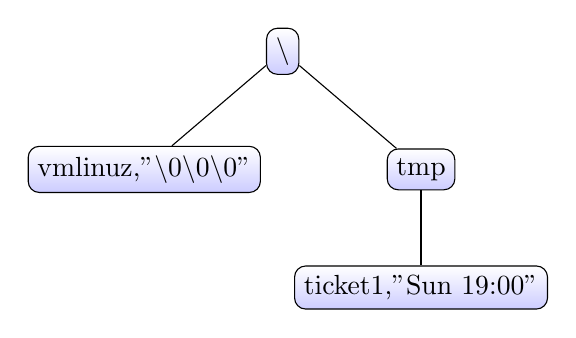
\begin{tikzpicture}[sibling distance=10em,
  every node/.style = {shape=rectangle, rounded corners,
    draw, align=center,
    top color=white, bottom color=blue!20}]
  \node {\textbackslash}
    child { node {vmlinuz,{"}\textbackslash0\textbackslash0\textbackslash0{"}} }
    child { node {tmp}
      child { node {ticket1,{"}Sun 19:00{"}}}};
\end{tikzpicture}
\end{frame}

\begin{frame}{Model 1}
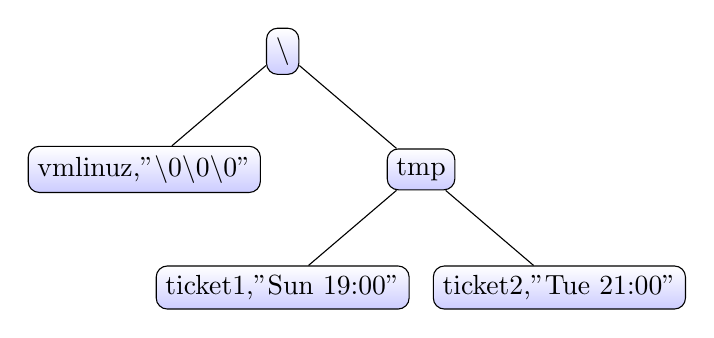
\begin{tikzpicture}[sibling distance=10em,
  every node/.style = {shape=rectangle, rounded corners,
    draw, align=center,
    top color=white, bottom color=blue!20}]
  \node {\textbackslash}
    child { node {vmlinuz,{"}\textbackslash0\textbackslash0\textbackslash0{"}} }
    child { node {tmp}
      child { node {ticket1,{"}Sun 19:00{"}}}
      child { node {ticket2,{"}Tue 21:00{"}}}};
\end{tikzpicture}
\end{frame}

\begin{frame}{Model 1}
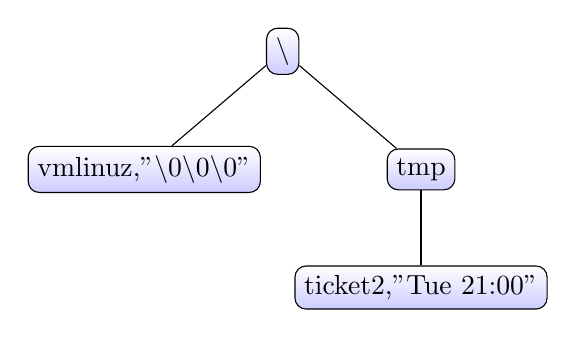
\begin{tikzpicture}[sibling distance=10em,
  every node/.style = {shape=rectangle, rounded corners,
    draw, align=center,
    top color=white, bottom color=blue!20}]
  \node {\textbackslash}
    child { node {vmlinuz,{"}\textbackslash0\textbackslash0\textbackslash0{"}} }
    child { node {tmp}
      child { node {ticket2,{"}Tue 21:00{"}}}};
\end{tikzpicture}
\end{frame}

\begin{frame}{Model 1}
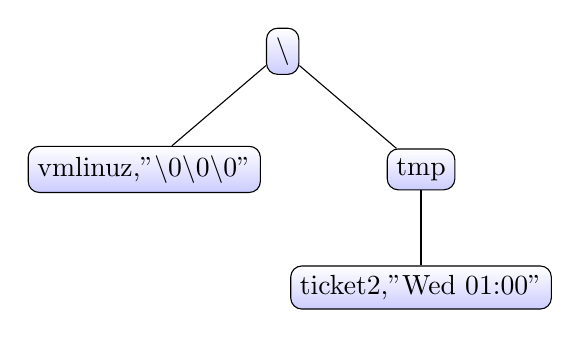
\begin{tikzpicture}[sibling distance=10em,
  every node/.style = {shape=rectangle, rounded corners,
    draw, align=center,
    top color=white, bottom color=blue!20}]
  \node {\textbackslash}
    child { node {vmlinuz,{"}\textbackslash0\textbackslash0\textbackslash0{"}} }
    child { node {tmp}
      child { node {ticket2,{"}Wed 01:00{"}}}};
\end{tikzpicture}
\end{frame}

\begin{frame}{Model 2}
  \begin{itemize}
  \item Model 1 supports nested directory structures, unbounded file
    size and unbounded filesystem size.
  \item However, there's no metadata, either to provide additional
    information or to validate the contents of the file.
  \item With an extra field for length, we can create a simple
    version of fsck that checks file contents for consistency.
  \item Further, we can verify that create, write, delete etc preserve
    this notion of consistency.
  \end{itemize}
\end{frame}

\begin{frame}{Model 2}
  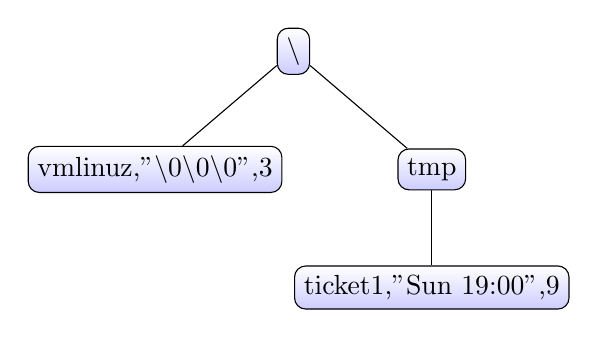
\begin{tikzpicture}[sibling distance=10em,
      every node/.style = {shape=rectangle, rounded corners,
        draw, align=center,
        top color=white, bottom color=blue!20}]]
      \node {\textbackslash}
      child { node {vmlinuz,{"}\textbackslash0\textbackslash0\textbackslash0{"},3} }
      child { node {tmp}
        child { node {ticket1,{"}Sun 19:00{"},9}}};
  \end{tikzpicture}
\end{frame}

\begin{frame}{Model 2}
  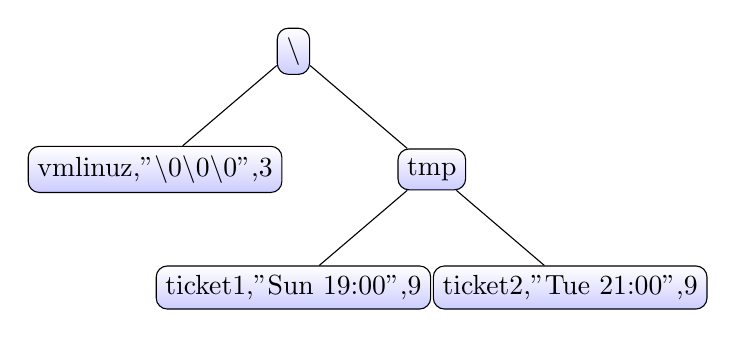
\begin{tikzpicture}[sibling distance=10em,
      every node/.style = {shape=rectangle, rounded corners,
        draw, align=center,
        top color=white, bottom color=blue!20}]]
      \node {\textbackslash}
      child { node {vmlinuz,{"}\textbackslash0\textbackslash0\textbackslash0{"},3} }
      child { node {tmp}
        child { node {ticket1,{"}Sun 19:00{"},9}}
        child { node {ticket2,{"}Tue 21:00{"},9}}};
  \end{tikzpicture}
\end{frame}

\begin{frame}{Model 2}
  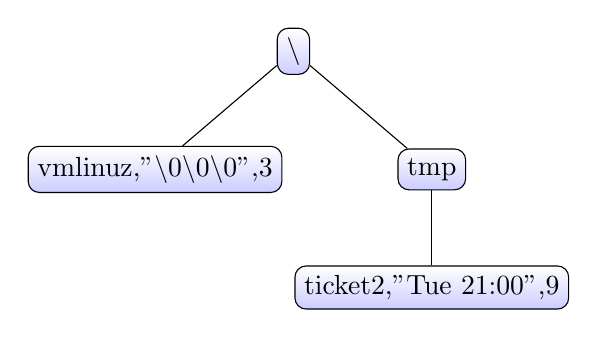
\begin{tikzpicture}[sibling distance=10em,
      every node/.style = {shape=rectangle, rounded corners,
        draw, align=center,
        top color=white, bottom color=blue!20}]]
      \node {\textbackslash}
      child { node {vmlinuz,{"}\textbackslash0\textbackslash0\textbackslash0{"},3} }
      child { node {tmp}
        child { node {ticket2,{"}Tue 21:00{"},9}}};
  \end{tikzpicture}
\end{frame}

\begin{frame}{Model 2}
  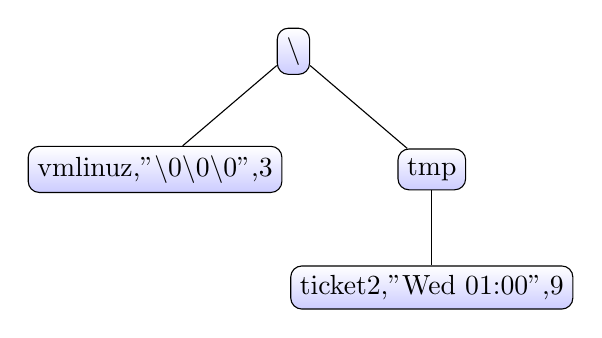
\begin{tikzpicture}[sibling distance=10em,
      every node/.style = {shape=rectangle, rounded corners,
        draw, align=center,
        top color=white, bottom color=blue!20}]]
      \node {\textbackslash}
      child { node {vmlinuz,{"}\textbackslash0\textbackslash0\textbackslash0{"},3} }
      child { node {tmp}
        child { node {ticket2,{"}Wed 01:00{"},9}}};
  \end{tikzpicture}
\end{frame}

\begin{frame}{Model 3}
  \begin{itemize}
  \item As the next step, we would like to begin externalising the
    storage of file contents.
  \item It would also be good to break up file contents into "blocks"
    of a finite length.
    \begin{itemize}
    \item Note: this would mean storing file length is no longer
      optional.
    \end{itemize}
  \end{itemize}
\end{frame}

\begin{frame}{Model 3}
  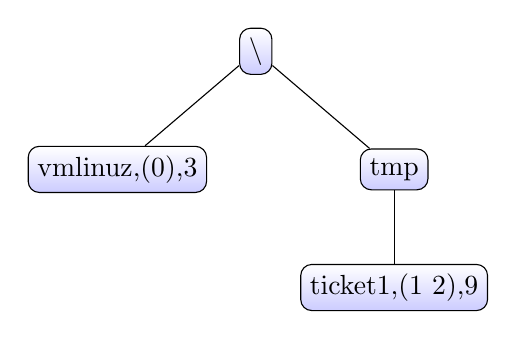
\begin{tikzpicture}[sibling distance=10em,
      every node/.style = {shape=rectangle, rounded corners,
        draw, align=center,
        top color=white, bottom color=blue!20}]]
      \node {\textbackslash}
      child { node {vmlinuz,(0),3} }
      child { node {tmp}
        child { node {ticket1,(1 2),9}}};
  \end{tikzpicture}
  \begin{table}[]
    %% \centering
    \caption{Disk}
    \label{my-label}
    \begin{tabular}{|l|}
      \hline
      \textbackslash0\textbackslash0\textbackslash0   \\ \hline
      Sun 19:0 \\ \hline
      0        \\ \hline
    \end{tabular}
  \end{table}
\end{frame}

\begin{frame}{Model 3}
  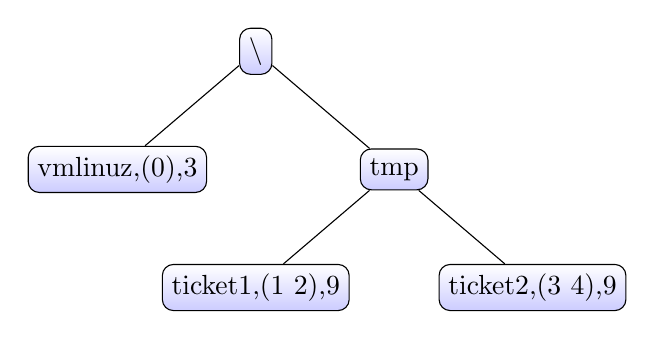
\begin{tikzpicture}[sibling distance=10em,
      every node/.style = {shape=rectangle, rounded corners,
        draw, align=center,
        top color=white, bottom color=blue!20}]]
      \node {\textbackslash}
      child { node {vmlinuz,(0),3} }
      child { node {tmp}
        child { node {ticket1,(1 2),9}}
        child { node {ticket2,(3 4),9}}};
  \end{tikzpicture}
  \begin{table}[]
    \centering
    \caption{Disk}
    \label{my-label}
    \begin{tabular}{|l|}
      \hline
      \textbackslash0\textbackslash0\textbackslash0   \\ \hline
      Sun 19:0 \\ \hline
      0        \\ \hline
      Tue 21:0 \\ \hline
      0        \\ \hline
    \end{tabular}
  \end{table}
\end{frame}

\begin{frame}{Model 3}
  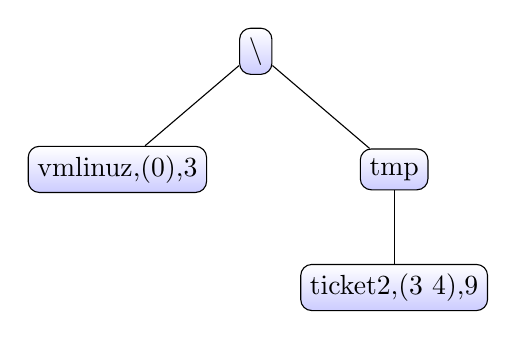
\begin{tikzpicture}[sibling distance=10em,
      every node/.style = {shape=rectangle, rounded corners,
        draw, align=center,
        top color=white, bottom color=blue!20}]]
      \node {\textbackslash}
      child { node {vmlinuz,(0),3} }
      child { node {tmp}
        child { node {ticket2,(3 4),9}}};
  \end{tikzpicture}
  \begin{table}[]
    \centering
    \caption{Disk}
    \label{my-label}
    \begin{tabular}{|l|}
      \hline
      \textbackslash0\textbackslash0\textbackslash0   \\ \hline
      Sun 19:0 \\ \hline
      0        \\ \hline
      Tue 21:0 \\ \hline
      0        \\ \hline
    \end{tabular}
  \end{table}
\end{frame}

\begin{frame}{Model 3}
  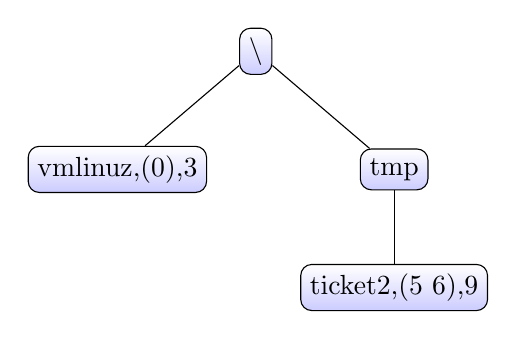
\begin{tikzpicture}[sibling distance=10em,
      every node/.style = {shape=rectangle, rounded corners,
        draw, align=center,
        top color=white, bottom color=blue!20}]]
      \node {\textbackslash}
      child { node {vmlinuz,(0),3} }
      child { node {tmp}
        child { node {ticket2,(5 6),9}}};
  \end{tikzpicture}
  \begin{table}[]
    \centering
    \caption{Disk}
    \label{my-label}
    \begin{tabular}{|l|}
      \hline
      \textbackslash0\textbackslash0\textbackslash0   \\ \hline
      Sun 19:0 \\ \hline
      0        \\ \hline
      Tue 21:0 \\ \hline
      0        \\ \hline
      Wed 01:0 \\ \hline
      0        \\ \hline
    \end{tabular}
  \end{table}
\end{frame}

\begin{frame}{Model 4}
  \begin{itemize}
  \item In the fourth model, we implement garbage collection in the
    form of an allocation vector.
  \item What guarantees do we need to show that a filesystem of this
    kind is consistent? (\textit{We'll return to this question.})
  \end{itemize}
\end{frame}

\begin{frame}{Model 4}
  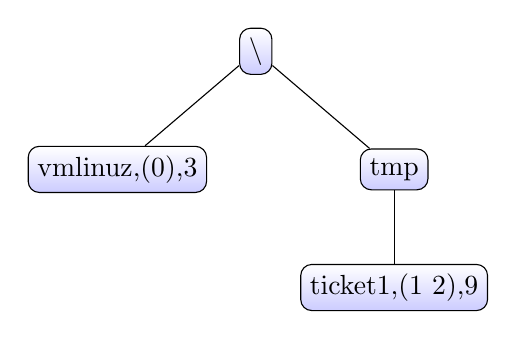
\begin{tikzpicture}[sibling distance=10em,
      every node/.style = {shape=rectangle, rounded corners,
        draw, align=center,
        top color=white, bottom color=blue!20}]]
      \node {\textbackslash}
      child { node {vmlinuz,(0),3} }
      child { node {tmp}
        child { node {ticket1,(1 2),9}}};
  \end{tikzpicture}
  \begin{table}[]
    %% \centering
    \caption{Disk}
    \label{my-label}
    \begin{tabular}{|l|}
      \hline
      \textbackslash0\textbackslash0\textbackslash0   \\ \hline
      Sun 19:0 \\ \hline
      0        \\ \hline
    \end{tabular}
  \end{table}
\end{frame}

\begin{frame}{Model 4}
  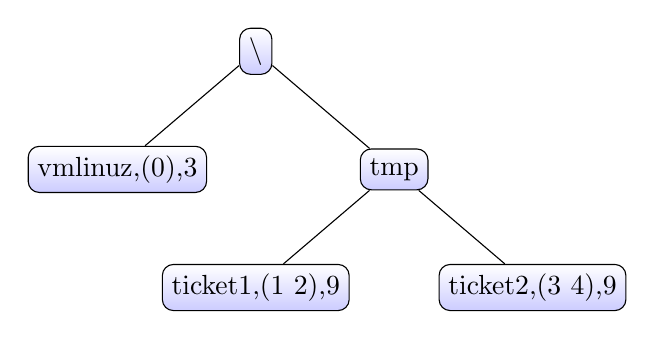
\begin{tikzpicture}[sibling distance=10em,
      every node/.style = {shape=rectangle, rounded corners,
        draw, align=center,
        top color=white, bottom color=blue!20}]]
      \node {\textbackslash}
      child { node {vmlinuz,(0),3} }
      child { node {tmp}
        child { node {ticket1,(1 2),9}}
        child { node {ticket2,(3 4),9}}};
  \end{tikzpicture}
  \begin{table}[]
    \centering
    \caption{Disk}
    \label{my-label}
    \begin{tabular}{|l|}
      \hline
      \textbackslash0\textbackslash0\textbackslash0   \\ \hline
      Sun 19:0 \\ \hline
      0        \\ \hline
      Tue 21:0 \\ \hline
      0        \\ \hline
    \end{tabular}
  \end{table}
\end{frame}

\begin{frame}{Model 4}
  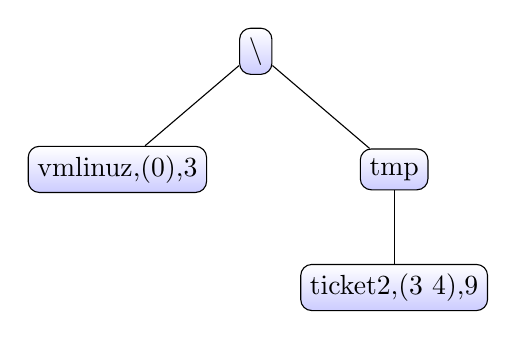
\begin{tikzpicture}[sibling distance=10em,
      every node/.style = {shape=rectangle, rounded corners,
        draw, align=center,
        top color=white, bottom color=blue!20}]]
      \node {\textbackslash}
      child { node {vmlinuz,(0),3} }
      child { node {tmp}
        child { node {ticket2,(3 4),9}}};
  \end{tikzpicture}
  \begin{table}[]
    \centering
    \caption{Disk}
    \label{my-label}
    \begin{tabular}{|l|}
      \hline
      \textbackslash0\textbackslash0\textbackslash0   \\ \hline
      Sun 19:0 \\ \hline
      0        \\ \hline
      Tue 21:0 \\ \hline
      0        \\ \hline
    \end{tabular}
  \end{table}
\end{frame}

\begin{frame}{Model 4}
  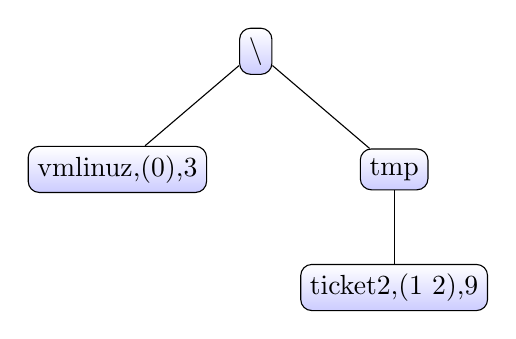
\begin{tikzpicture}[sibling distance=10em,
      every node/.style = {shape=rectangle, rounded corners,
        draw, align=center,
        top color=white, bottom color=blue!20}]]
      \node {\textbackslash}
      child { node {vmlinuz,(0),3} }
      child { node {tmp}
        child { node {ticket2,(1 2),9}}};
  \end{tikzpicture}
  \begin{table}[]
    \centering
    \caption{Disk}
    \label{my-label}
    \begin{tabular}{|l|}
      \hline
      \textbackslash0\textbackslash0\textbackslash0   \\ \hline
      Wed 01:0 \\ \hline
      0        \\ \hline
      Tue 21:0 \\ \hline
      0        \\ \hline
    \end{tabular}
  \end{table}
\end{frame}

\section{Progress so far}
\begin{frame}{Proof approaches and techniques}
  \begin{itemize}
  \item There are many properties that could be considered for
    correctness, but the read-over-write theorems from the first-order
    theory of arrays seem like a good place to start.
    \begin {enumerate}
    \item Reading from a location after writing to the same location
      should yield the data that was written. Formally, assuming \texttt{n =
      length(text)} and suitable "type" hypotheses (omitted here): \\
      \texttt{l1-rdchs(hns, l1-wrchs(hns, fs, start, text), start, n)
      =
      text}
    \item Reading from a location after writing to a different
      location should yield the same result as reading before
      writing. Formally, assuming \texttt{hns1 != hns2} and suitable "type"
      hypotheses (omitted here):\\
      \texttt{l1-rdchs(hns1, l1-wrchs(hns2, fs, start2, text2), start1, n1)
        =
        l1-rdchs(hns1, fs, start1, n1)}
    \end {enumerate}
    \item For each of the models 1, 2 and 3, we have proofs of correctness of
      the two read-after-write properties, based on the proofs of
      equivalence between each model and its successor.
  \end{itemize}
\end{frame}

\begin{frame}{Proof approaches and techniques}
  \begin{enumerate}
  \item For model 4, the disk and the allocation vector must be in harmony
    initially and updated in lockstep.
  \item Every block referred to in the filesystem must be marked
    "used" in the allocation vector.\\
    (The complementary problem - making sure unused
      blocks are unmarked - is more complicated because it's non-local.)
  \item If n blocks are available in the allocation vector, the
    allocation algorithm must provide n blocks when requested.
  \item No matter how many blocks are returned by the allocation
    algorithm, they must be unique and disjoint with the blocks
    allocated to other files.
  \end{enumerate}
\end{frame}

\section{Future work}

\begin{frame}{Permissions}
  \begin{itemize}
  \item What does permission checking look like in ACL2?
  \item Top-down: picture the theorems that would prove correctness.
    \begin{enumerate}
    \item Read/write/execute permission is granted when the requesting
      user has permission for themselves/their group, or when the
      permission is granted to all.
    \item Converse: read/write/execute permission is denied when none
      of the above hold.
    \item Reads that fail because of permissions do not return a value.
    \item Writes that fail because of permissions return an unmodified
      filesystem.
    \end{enumerate}
  \item Gee, how do we represent users and groups?
    \begin{enumerate}
    \item Users are natural numbers.
    \item Groups are also natural numbers, and a vector (psst: a
      nat-list) holds the group associated with each user.
    \end{enumerate}
  \end{itemize}
\end{frame}

\begin{frame}{Other future work}
  \begin{itemize}
  \item Finish read-over-write proofs for model 4.
  \item Possibly, add the system call open and close with the
    introduction of file descriptors.\\
    \textit{This would be a step towards the study of concurrent FS operations.}
  \item Linearise the tree, leaving only the disk.
  \item Eventually emulate the CP/M filesystem as a convincing proof
    of concept, and move on to fsck and file recovery tools.
  \end{itemize}
\end{frame}

\end{document}
